\documentclass[10pt,a4paper]{article}
\usepackage{graphicx}
\usepackage{changepage}
\usepackage{amsmath}
\usepackage{mathtools}
\usepackage{hyperref}
\usepackage{enumitem}
\begin{document}

%\newcommand{\eActTrainSensData(ARRIVE)}[1]{\texttt{eActTrainSensData(ARRIVE,#1)}}
%\newcommand{\eActTrainSensData(LEFT)}[1]{\texttt{eActTrainSensData(LEFT,#1)}}
%\newcommand{\eActTrainSensData(BREAK)}[1]{\texttt{eActTrainSensData(BREAK,#1)}}
% \newcommand{\eActSetBarrier(OPEN)}{\texttt{eActSetBarrier(OPEN)}}
% \newcommand{\eActSetBarrier(CLOSE)}{\texttt{eActSetBarrier(CLOSE)}}
% \newcommand{\eActSetSignal(GREEN)}{\texttt{eActSetSignal(GREEN)}}
% \newcommand{\eActSetSignal(RED)}{\texttt{eActSetSignal(RED)}}
% \newcommand{\eActSetSignal(YELLOW)}{\texttt{eActSetSignal(YELLOW)}}
% \newcommand{\eActSetWarnLight(W\_LOW)}{\texttt{eActSetWarnLight(W\_LOW)}}
% \newcommand{\eActSetWarnLight(W\_HIGH)}{\texttt{eActSetWarnLight(W\_HIGH)}}
% \newcommand{\eActSetWarnLight(W\_OFF)}{\texttt{eActSetWarnLight(W\_OFF)}}
% \newcommand{\eActSetTime(time1)}{\texttt{eActSetSignal(time1)}}
% \newcommand{\eActSetTime(time2)}{\texttt{eActSetSignal(time2)}}
% \newcommand{\eActSetTime(time3)}{\texttt{eActSetSignal(time3)}}
% \newcommand{\RESET}{\texttt{RESET}}
% \newcommand{\MANUAL_FIX}{\texttt{MANUAL_FIX}}
% \newcommand{\RESET_COMPLETE}{\texttt{RESET_COMPLETE}}
% \newcommand{\eActGetSpeed(s)}{\texttt{eActGetSpeed(s)}}


\title{\Huge{\textbf{System Validation\\ Final Report\\[3cm]}}} % change later%

\author{\LARGE{Pablo Martin Guijo (0976197)}\\
	\LARGE{Sri Muthu Narayanan Balasubramanian (0978367)}\\
	\LARGE{Nitesh Agarwal (0981729)}\\
	\LARGE{Prathyusha Adiraju (0977176)}\\[5cm]
	}

\date{\Large{October 23th 2015\\Version 2.0\\}}
\maketitle

\newpage
%------------------------------------------------------------------
% Contents%
%------------------------------------------------------------------
\tableofcontents
\newpage

\section{Revision History}
After the first review, the following changes have been made in accordance with the comments from Prof.J.F.Groote.
\begin{enumerate}
\item Figure 1 was modified to include the Controller block.
\item Sections 2.1 and 3 - Explanation for the status of assumption and requirements was added respectively.
\item Section 5.2, Requirement \#6, footnote added for clarity.
\item Section 8.1, Requirements \#4 and \#5, $\cap$ was replaced with $\wedge$
\item Section 8.2, Requirement \#8 was rewritten.
\item Section 9, Details of verification setup added.
\item Punctuation errors rectified throughout the report.

\end{enumerate}
%------------------------------------------------------------------
% Introductiong Section%
%------------------------------------------------------------------
\newpage
\section{Introduction}

The purpose of this document is to design and validate an Automated Railroad Crossing System (ARCS). The goal of the system is to provide a fully automated and failsafe method for monitoring a railroad intersection to avoid accidents. \\
The primary functionality of the system is to monitor the intersection for the arrival and departure of trains using an array of train sensors on either side of the intersection and actuate the traffic signals, barriers, warning lights and alarms based on the data from the train sensors. The system also takes into account the failure of a train monitoring sensor, which is treated as a critical failure causing the system to enter the fail-safe mode, thereby closing the barriers and switching the signals to red until the sensors are replaced and the system is reset manually.\\
The system determines the speed at which the trains approach the intersection and computes the reaction time after which the signals switch and the barriers close. When  multiple trains approach the intersection, the response time is determined by the earliest timer that expires. When two or more trains approach the intersection in a sequence, the behavior is designed such that only after all the trains that approach the intersection leave, the barriers open and the signals are switched to green. The rest of the document gives a formal description of the system, the system model and the verification of the requirements using the mCRL2 toolset. The complete model of the system is also presented.

   \begin{figure}[thpb]
      \centering
      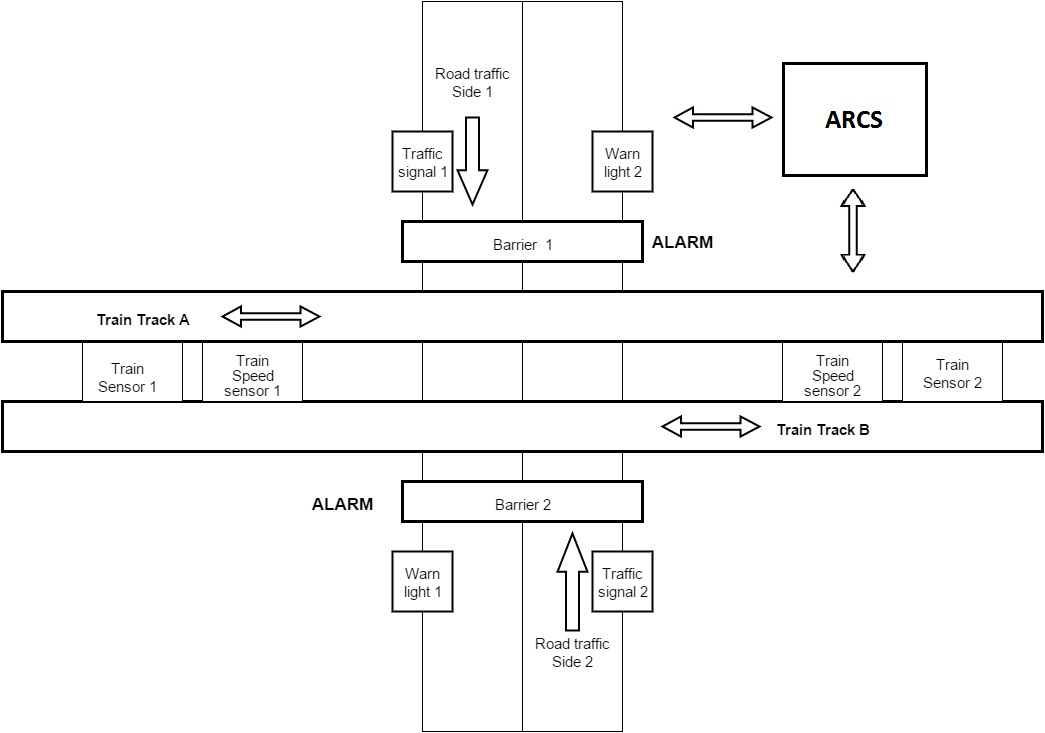
\includegraphics[scale=0.6]{Sys_Val_D2.jpg}
      \caption{System Schematic Diagram}
      \label{figurelabel}
   \end{figure}

%------------------------------------------------------------------
% Assumptions%
%------------------------------------------------------------------
%\newpage
%
%\subsection{Flow Table}
%	\begin{table}[!hbp]
%	\centering
%	\begin{adjustwidth}{-2.4cm}{}
%	\begin{tabular}{|l|l|l|l|l|l|l|l|}
%	\hline
%&\textbf{Conceptual}&\textbf{Train}&\textbf{AfterT1}&\textbf{AfterT2}&\textbf{AfterT4}&\textbf{After}&\textbf{AfterT3}\\
%    &\textbf{initial state}&\textbf{Arrives}&&&&\textbf{trains leave}&\\
%    \hline
%    \textbf{Traffic}&GREEN&YELLOW&RED&RED&RED&RED&GREEN\\
%    \textbf{Light}&&&&&&&\\
%    \hline
%    \textbf{Warning}&OFF&LOW&HIGH&HIGH&HIGH&HIGH&OFF\\
%    \textbf{Light}&&&&&&&\\
%    \hline
%    \textbf{Bell}&OFF&OFF&ON&ON&ON&ON&OFF\\
%    \hline
%    \textbf{Barrier}&OPEN&OPEN&OPEN&Starts to&CLOSED&Starts to&OPEN\\
%    &&&&CLOSE&&OPEN&\\
%    \hline
%    
%	\end{tabular}
%	\end{adjustwidth}
%	\caption{Table illustrating the process flow}
%	\end{table}
    
\subsection{Assumptions}
In order to allow for a more complete design of the system, reducing complexity and allowing easy testability, the assumptions below were made. These assumptions represent behaviours of the system that our controller will not have to prove as they are supposed to be true.
\begin{enumerate}
\item Two or more trains cannot arrive at the intersection at the exact same moment.
\item When a third train arrives at the intersection the barriers will have already been closed.
\item No Signals or warning lights can change, unless the ARCS's system commands the signals to change.
\item In case of any sensor failure, the sensors will be fixed manually. No trains can arrive at the intersection at the time when Manual Reset is being done after the Manual fix.
\item \textbf{The conceptual initial state} is defined as the state in which no trains have arrived, the traffic lights are green, warning lights are off, barriers are open and the bell is off.
\end{enumerate}

    
%------------------------------------------------------------------
% List of requirements%
%------------------------------------------------------------------

\newpage

\section{List of requirements}
List of general requirements specify the behavior of the system described in the introduction. The ARCS controller is designed to verify all of them. These requierements are classified based on different parts of the system, i.e., sensors, signals, bell and barriers.
\subsection{Sensors}
\begin{enumerate}
\item A sensor break can be detected at all times except, in between a sensor break and a system reset.
\item When a sensor breaks, eventually, the signals will turn ``Red'', the warning lights will ``Flash High'', the bell will Turn ``On'' and the Barriers will close.
\item After a sensor breaks and the barriers close, they will remain closed until the sensor is fixed and the system is manually reset.
\item When the system is not in the conceptual initial state, when a train arrives and the signals are green, the speed of the train is acquired, unless another train arrives or a sensor break happens in between.
\item When the train arrives and the system is in the conceptual initial state, the speed of the train is acquired unless another train arrives or a sensor break happens in between.

\end{enumerate}
\subsection{Signals}
\begin{enumerate}[resume]
\item When a train approaches and there is no train at the intersection, eventually, the traffic lights should turn ``Yellow'' and the Warning lights should ``Flash Low''.
\item When a train approaches and there is a train already present at the intersection, traffic lights will turn ``Yellow'' eventually, if they have not already turned ``Yellow''.
\item When a train approaches and there is a train already present at the intersection, warning lights will ``Flash Low'' eventually, if they are already not ``Flashing Low''.
\item When the timer T1 expires, eventually, traffic lights must turn ``Red'' and the warning lights must ``Flash High''.
\item Before the barriers are closed, the traffic lights must be ``Red'' and the warning lights must be ``Flashing High''.
\item The traffic lights must remain ``Red'' and the warning lights must remain ``Flashing High'' as long as the barriers are closed.
\item After a reset, traffic lights must eventually turn ``Green'' and the warning lights must eventually turn ``Off''.
\item When the timer T3 expires, the traffic lights must eventually turn ``Green'' and the warning lights must eventually turn ``Off''.
\item The traffic lights must never go from ``Red'' to ``Yellow'' without going through ``Green'' and warning lights must never go from ``High'' to ``Low'' without going through ``Off''.
\item The traffic lights must never go from ``Yellow'' to ``Green'' without going through ``Red'' and warning lights must never go from ``Low'' to ``Off'' without going through ``High''.
\end{enumerate}

\subsection{Bell}
\begin{enumerate}[resume]
\item Before the barriers are closed, the bell must be ``On''.
\item The bell must remain ``On'' as long as the barriers are closed.
\item The bell is eventually turned ``Off'' when the barriers are opened.
\end{enumerate}

\subsection{Barriers}
\begin{enumerate}[resume]
\item The barriers must eventually close after the traffic lights turn ``Red''.
\item The barriers must eventually open after a reset.
\item The barriers must open when every train that approached the intersection has left the intersection.
\end{enumerate}

\subsection{Deadlock}
\begin{enumerate}[resume]
\item The system must be deadlock free.
\end{enumerate}


%------------------------------------------------------------------
% List of external actions%
%------------------------------------------------------------------
\newpage
\section{List of external actions}

The following table shows a list of all the external actions \textbf{\textit{of the control system.}}\\

\begin{table}[!hbp]
	\centering
	\begin{adjustwidth}{-1.5cm}{}
	\begin{tabular}{|c|l|l|c|}
		\hline 
		\textbf{No.} & \textbf{Name (data type)
        }&\textbf{Description} & \textbf{flow} \\
		\hline
         E1&eActTrainSensData&Notifies the status and number of trains.&INPUT\\
         &(status,TrainNo)& Status can be arrives, leaves or broken. & \\
         & & TrainNo is \textbf{the number of trains in the intersection} &\\
         && \textbf{at any given time after this action takes place}.&\\ &&It is -1 when the sensor is broken & \\
         \hline
         E2&eActSetBarrier(status)&Commands the barriers to be in the given status.&OUTPUT\\
         &&Status can be open or close.& \\
         \hline
         E3&eActSetBell(status)&Commands the bell to be in the given status.&OUTPUT\\ 
         &&Status can be on or off.&\\
         \hline
         E4&eActSetSignal(status)&Commands the traffic signals to be in the given status.&OUTPUT\\
         &&Status can be green, yellow or red.&\\
         \hline
         E5&eActSetWarnLight&Commands the warning lights to be in the given status.&OUTPUT\\
         &(status)&Status can be high, low or off.&\\
         \hline
         E6&eActTime(time)&Notifies when the timer has expired.&INPUT\\
         &&Time can be: time1, time2, time3, time4, &\\
         &&notime, t0, t1, t2, t3, t4 , t5&\\
         \hline
         E7&RESET&The reset action occurs to move the system&INPUT\\
         &&to the conceptual initial state.&\\
         \hline
         E8&MANUAL\_FIX&Notifies when the sensor is broken and needs a&INPUT\\
         &&manual fix.&\\
         \hline
         E9&RESET\_COMPLETE& Notifies that the system reset is complete&INPUT\\
         &&and system returns to conceptual initial state.&\\
         \hline
         E10&eActGetSpeed(speed)&Gets the train speed  &INPUT\\
         &&speed can be s0, s1, s2, s3, s4, s5, noSpeed&\\   
         \hline
         		\end{tabular}
				\end{adjustwidth}
	\caption{List of external actions}
\end{table}
\textbf{Note:}
\\ \textit{time1} is the time to wait between the traffic signals turn yellow to the time they turn red
\\ \textit{time2} is time to wait between the traffic signals turn red and the start of closing the barrier.
\\ \textit{time3} is the time the barrier needs to open.\\time4 is the time the barrier needs to close.
\\ \textit{notime} means that an action is imminent.
\\ \textit{t0 to t5} denote the time intervals that the system must wait depending on the speed read.
% Insert graphic%
% \begin{figure}[h]
% 	\centering
% 	\includegraphics[scale=0.9]{pictures/drawing1.pdf}
% 	\caption{An overview of the external actions and their directions}
% \end{figure}


\clearpage

\newpage

%------------------------------------------------------------------
%Requirements in term of action
%------------------------------------------------------------------
\section{Requirements expressed in terms of actions}

In this section, the requirements listed in section 2 will be translated in terms of the actions described in section 3. \\
%\textit{f,f1,f2,fOld: Freq} \\
%\textit{v,v1,v2: Speed} \\
\subsection{Sensors}
\begin{enumerate}
\item 
	\begin{enumerate}
	\item If a first \textbf{eActTrainSensData(BREAK,-1)} has not happened, it can happen at any state.
	\item After any \textbf{eActTrainSensData(BREAK,-1)},\\ another \textbf{eActTrainSensData(BREAK,-1)} can happen again only after a \textbf{RESET\_COMPLETE.}
    \item Between a \textbf{eActTrainSensData(BREAK,-1)} and a \textbf{RESET\_COMPLETE} an \textbf{eActTrainSensData(BREAK,-1)} cannot happen.
	\end{enumerate}
\item After an \textbf{eActTrainSensData(BREAK,-1)} happens, after a finite number of steps, \textbf{eActSetSignal(RED),  eActSetWarnLight(HIGH), eActSetBell(BELL\_ON)} and \textbf{eActSetBarrier(CLOSE)} will take place.
\item After a \textbf{eActTrainSensData(BREAK,-1)}, an \textbf{eActSetBarrier(OPEN)} cannot happen until \textbf{RESET} happens.
\item When an \textbf{eActSetSignal(GREEN)} happens not followed by \textbf{eActSetSignal(YELLOW)} or \textbf{eActSetSignalAction(RED)} and an \textbf{eActTrainSensData(ARRIVE,1)} happens, \textbf{eActGetTrainSpeed} action takes place unless an \textbf{eActTrainSensData(ARRIVE,2)} happens or\\ \textbf{eActTrainSensData(BREAK,-1)} occurs in between.
\item When \textbf{eActTrainSensData(ARRIVE,1)} takes place \textbf{eActGetTrainSpeed} action occurs unless an \textbf{eActTrainSensData(ARRIVE,2)} happens or \textbf{eActTrainSensData(BREAK,-1)} occurs in between.
\end{enumerate}

\subsection{Signals}
\begin{enumerate}[resume]
\item When \textbf{eActTrainSensData(ARRIVE,1)}\footnote{ - The number 1 denotes that after this action happens, there will be 1 train in the intersection. Therefore, this means that it is the first train to approach the intersection} happens, an \textbf{eActSetSignal(YELLOW)} will follow , after a finite number of steps.
\item When \textbf{eActTrainSensData(ARRIVE,2)} happens, \textbf{eActSetSignal(YELLOW)} will happen after a finite number of steps, if it has not already happened.
\item When \textbf{eActTrainSensData(ARRIVE,2)} happens, an \textbf{eActSetWarnLight (W\_LOW)} will follow, after a finite number of steps, if it has not already happened.
\item After \textbf{eActTime(time1)} expires, an \textbf{eActSetSignal(RED)} and \textbf{eActSetWarnLight(W\_HIGH)} must happen, after a finite number of steps.
\item  Every \textbf{eActSetBarrier(CLOSE)} must be preceded by an \textbf{eActSetSignal(RED)} and \textbf{eActSetWarnLight(W\_HIGH)}, without \textbf{eActSetWarnLight(W\_OFF)} or \textbf{eActSetWarnLight(W\_LOW)} or \textbf{eActSetSignal(GREEN)} or \textbf{eActSetSignal(YELLOW)}happening in between.
\item In between \textbf{eActSetBarrier(CLOSE)} and \textbf{eActSetBarrier(OPEN)} the actions \textbf{eActSetWarnLight(W\_OFF)} or \textbf{eActSetWarnLight(W\_LOW)}or \textbf{eActSetSignal(GREEN)} or \textbf{eActSetSignal(YELLOW)} cannot take place.
\item After a \textbf{RESET} action happens, \textbf{eActSetSignal(GREEN)} and \textbf{eActSetWarnLight(OFF)} should happen  , in a finite number of steps.
\item After \textbf{eActTime(time3)} expires, \textbf{eActSetSignal(GREEN)} and \textbf{eActSetWarnLight(OFF)} should happen, in a finite number of steps
\item Between actions \textbf{eActSetSignal(RED)} and \textbf{eActSetSignal(GREEN)} an \textbf{eActSetSignal(YELLOW)} should not take place and between \textbf{eActSetWarnLight(W\_HIGH)} and \textbf{eActSetWarnLight(W\_OFF)} an \textbf{eActSetWarnLight(W\_LOW)} should not take place.
\item Between actions \textbf{eActSetSignal(YELLOW)} and \textbf{eActSetSignal(RED)} an \textbf{eActSetSignal(GREEN)} should not take place and between \textbf{eActSetWarnLight(W\_LOW)} and \textbf{eActSetWarnLight(W\_HIGH)} an \textbf{eActSetWarnLight(W\_OFF)} should not take place.
\end{enumerate}

\subsection{Bell}
\begin{enumerate}[resume]
\item Every \textbf{eActSetBarrier(CLOSE)} must be preceded by an \textbf{eActSetBell(BELL\_ON)}, without \textbf{eActSetBell (BELL\_OFF) }happening in between.
\item In between \textbf {eActSetBarrier(CLOSE) }and \textbf{eActSetBarrier(OPEN)} the actions \textbf {eActSetBell (BELL\_OFF)} cannot take place.
\item After \textbf{eActSetBarrier(OPEN) }takes place, an \textbf{eActSetBell(OFF)} must happen, in a finite number of steps.
\end{enumerate}

\subsection{Barriers}
\begin{enumerate}[resume]
\item After \textbf{eActSetSignal(RED)} takes place, the \textbf{eActSetBarrier(CLOSE)} should take place in a finite number of steps.
\item After a \textbf{RESET} action takes place an \textbf{eActSetBarrier(OPEN)} must take place in a finite number of steps.
\item After \textbf{eActTrainSensData(LEFT,0)} an \textbf{eActSetBarrier(OPEN)} must happen in a finite number of steps.
\end{enumerate}

\subsection{Deadlock}
\begin{enumerate}[resume]
\item The system must be deadlock free.
\end{enumerate}

\newpage
%------------------------------------------------------------------
\section{Architecture}
%------------------------------------------------------------------
ARCS is designed to have three parallel components namely ARCS-TRAIN, ARCS-BARRIER and the ARCS-SIGNALS.\\
\\ The ARCS TRAIN handles the data from train monitoring sensors and updates the other two components when trains arrive or leave the intersection. The component also sends a notification when the sensor breaks. The data from the train speed sensors are also handled by the ARCS TRAIN component and this data is used to determine the time information needed for the co-ordination of the signals and barriers.\\
\\The ARCS BARRIER component is receives the notifications form ARCS TRAIN and ARCS SIGNALS, using the data to control the opening and closing of the barriers.\\
\\The ARCS SIGNALS component controls the traffic lights, warning lights and the alarm based on the notifications from ARCS TRAIN and ARCS BARRIER.

\newpage

%------------------------------------------------------------------
\section{List of internal actions}
%------------------------------------------------------------------
The following table shows all the internal actions together with a short description and the both the source and destination component:


\begin{table}[!hbp]
	\centering
	\begin{adjustwidth}{-2.3cm}{}
	\begin{tabular}{|l|l|l|l|l|}
		
		\hline
		\textbf{No.} & \textbf{Name} & \textbf{Description} & \textbf{Source} & \textbf{Dest} \\
		\hline
        I1& iActTrainsLeft &Notifies that the trains have left and the barriers&Train & Barrier\\
        &&can be opened & & \\ 
        \hline
        I2& iActResetBarrier& Notifies the system to reset to the conceptual initial&Train&Barrier\\
        &&state & &\\
        \hline
        I3& iActBarrierClose& Notifies that the barriers are closed & Barrier &Train\\
        \hline
        I4& iActTrainArrive&Notifies if a train has arrived & Train&Signals\\
        \hline
        I5& iActSendBreakSignals& Notifies that a sensor break has occurred& Train&Signals\\
        \hline
         I6& iActSignGreen& Notifies that the signals are green&Signals&Train\\ 
        \hline
         I7& iActBarrierOpen&Notifies that the trains have left  & Barrier&Signals\\
         &&and the barriers can be opened & &\\
        \hline
         I8& iActTimeBarrier& Notifies when the time expires, the signals are red& Signals&Barrier\\
        && and the barriers can be closed & &\\
        \hline
        
	
	\end{tabular}
	\end{adjustwidth}
	\caption{List of external actions}
\end{table}

\begin{figure}[thpb]
	\centering
	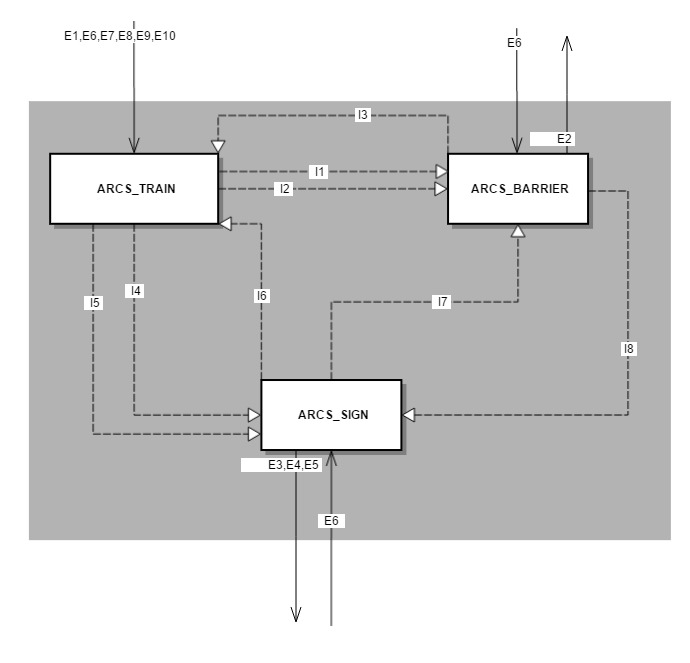
\includegraphics[scale=0.35]{Internal_Diag.JPG}
	\caption{An overview of the internal architecture and communications}
\end{figure} 

Note that the numbers in Figure 2 refer to the internal and external actions in tables 2 and 3

\newpage

\section{Requirements expressed in modal formulas}


This section contains a list of the initial requirements translated into modal formulas:
\subsection{Sensors}
\begin{enumerate}
\item 
	\begin{enumerate}
    \item $[\overline{eActTrainSensData(BREAK,-1)}^*]\langle eActTrainSensData(BREAK,-1) \rangle true$
    \item $[true*.RESET\_COMPLETE.\overline{eActTrainSensData(BREAK,-1)}^*] $\\$ \langle eActTrainSensData(BREAK,-1) \rangle true $
    \item $[true*.eActTrainSensData(BREAK,-1).\overline{RESET\_COMPLETE}^*. $\\$ eActTrainSensData(BREAK,-1)]false$
    \end{enumerate}
\item
	\begin{enumerate}
    \item $[true*.eActTrainSensData(BREAK,-1)]\mu X([\overline{eActSetSignal(RED)}]X \wedge \langle true\rangle  true)$
    \item $[true*.eActTrainSensData(BREAK,-1)]\mu X([\overline{eActSetWarnLight(W\_HIGH)}]X \wedge \langle true\rangle  true)$
    \item $[true*.eActTrainSensData(BREAK,-1)]\mu X([\overline{eActSetBell(BELL\_ON)}]X \wedge \langle true\rangle  true)$
    \item $[true*.eActTrainSensData(BREAK,-1)]\mu X([\overline{eActSetBarrier(CLOSE)}]X \wedge \langle true\rangle  true)$
    \end{enumerate}
\item $[true*.eActTrainSensData(BREAK,-1).\overline{RESET}^*.eActSetBarrier(OPEN)]false$
\item $[true*.eActSetSignal(GREEN).\overline{eActSetSignal(YELLOW) \cup eActSetSignal(RED)}^*. $\\$ eActTrainSensData(ARRIVE,1)]\mu X.([\forall _{s:Speed}.\overline{eActGetSpeed(s) } \cap  $\\$  \overline{ eActTrainSensData(BREAK,-1) } \cap \overline{ eActTrainSensData(ARRIVE,2) }]X \wedge  $\\$  \langle true \rangle true )$
\item $[eActTrainSensData(ARRIVE,1)]\mu X.([\forall _{s:Speed}.\overline{eActGetSpeed(s) } \cap  $\\$  \overline{ eActTrainSensData(BREAK,-1) } \cap \overline{eActTrainSensData(ARRIVE,2)}]X \wedge  $\\$ \langle true \rangle true )$
\end{enumerate}

\subsection{Signals}
\begin{enumerate}[resume]
\item
	\begin{enumerate}
    \item $[true*.eActTrainSensData(ARRIVE,1)]\mu X.([\overline{eActSetSigna(YELLOW)}]X \wedge \langle true\rangle  true)$
    \item $[true*.eActTrainSensData(ARRIVE,1)]\mu X.([\overline{eActSetWarnLight(W\_LOW)}]X \wedge \langle true\rangle	true)$
    \end{enumerate}
\item
$[\overline{eActSetSignal(YELLOW)}^*.eActTrainSensData(ARRIVE,2)] $\\$ \mu X.([\overline{eActSetSignal(YELLOW)}]X \wedge \langle true\rangle  true)$

\item $[\overline{eActSetWarnLight(W\_LOW)}^*.eActTrainSensData(ARRIVE,2)] $\\$ \mu X.([\overline{eActSetWarnLight(W\_LOW)}]X \wedge \langle true\rangle  true)$

\item
	\begin{enumerate}
    \item $[true*.eActTime(time1)]\mu X.([\overline{eActSetSignal(RED)}]X \wedge \langle true\rangle  true)$

	\item $[true*.eActTime(time1)]\mu X.([\overline{eActSetWarnLight(W\_HIGH)}]X \wedge \langle true\rangle  true)$
	\end{enumerate}
\item
	\begin{enumerate}
    \item $[\overline{eActSetSignal(RED)}^*.eActSetBarrier(CLOSE)]false$
	\item $[true*.eActSetSignal(GREEN).\overline{eActSetSignal(RED)}^*. $\\$ eActSetBarrier(CLOSE)]false$
	\item $[true*.eActSetSignal(YELLOW).\overline{eActSetSignal(RED)}^*. $\\$ eActSetBarrier(CLOSE)]false$
    \item $[\overline{eActSetWarnLight(W\_HIGH)}^*.eActSetBarrier(CLOSE)]false$
	\item $[true*.eActSetWarnLight(W\_OFF).\overline{eActSetWarnLight(W\_HIGH)}^*. $\\$ eActSetBarrier(CLOSE)]false$
	\item $[true*.eActSetWarnLight(W\_LOW).\overline{eActSetWarnLight(W\_HIGH)}^*. $\\$ eActSetBarrier(CLOSE)]false$
    \end{enumerate}
\item
	\begin{enumerate}
    \item $[true*.eActSetBarrier(CLOSE).\overline{eActSetBarrier(OPEN)}^*. $\\$ eActSetSignal(GREEN)]false$
	\item $[true*.eActSetBarrier(CLOSE).\overline{eActSetBarrier(OPEN)}^*. $\\$ eActSetSignal(YELLOW)]false$
    \item $[true*.eActSetBarrier(CLOSE).\overline{eActSetBarrier(OPEN)}^*. $\\$ eActSetWarnLight(W\_OFF)]false$
	\item $[true*.eActSetBarrier(CLOSE).\overline{eActSetBarrier(OPEN)}^*. $\\$ eActSetWarnLight(W\_LOW)]false$
    \end{enumerate}
\item
	\begin{enumerate}
    	\item $[true*.RESET]\mu X.([\overline{eActSetSignal(GREEN)}]X \wedge \langle true\rangle  true)$
		\item  $[true*.RESET]\mu X.([\overline{eActSetWarnLight(W\_OFF)}]X \wedge \langle true\rangle  true)$
    \end{enumerate}
\item
	\begin{enumerate}
		\item $[true*.ActTime(time3)]\mu X.([\overline{eActSetSignal(GREEN)}]X \wedge \langle true\rangle  true)$
		\item $[true*.eActTime(time3)]\mu X.([\overline{eActSetWarnLight(W\_OFF)}]X \wedge \langle true\rangle  true)$
    \end{enumerate}
\item
	\begin{enumerate}
		\item $[true*.eActSetSignal(RED).\overline{eActSetSignal(GREEN)}^*. $\\$ eActSetSignal(YELLOW)]false$
		\item $[true*.eActSetWarnLight(W\_HIGH).\overline{eActSetWarnLight(W\_OFF)}^*. $\\$ eActSetWarnLight(W\_LOW)]false$
	\end{enumerate}
\item
	\begin{enumerate}
	\item $[true*.eActSetSignal(YELLOW).\overline{eActSetSignal(RED)}^*. $\\$ eActSetSignal(GREEN)]false$
	\item $[true*.eActSetWarnLight(W\_LOW).\overline{eActSetWarnLight(W\_HIGH)}^*. $\\$ eActSetWarnLight(W\_OFF)]false$
	\end{enumerate}
\end{enumerate}
\subsection{Bell}
\begin{enumerate}[resume]
\item 
	\begin{enumerate}
    \item $[\overline{eActSetBell(BELL\_ON)}^*.eActSetBarrier(CLOSE)]false$
    \item $[true*.eActSetBell(BELL\_OFF).\overline{eActSetBell(BELL\_ON)}^*. $\\$ eActSetBarrier(CLOSE)]false$
    \end{enumerate}
\item $[true*.eActSetBarrier(CLOSE).\overline{eActSetBarrier(OPEN)}^*. $\\$ eActSetBell(BELL\_OFF)]false$
\item $[true*.eActSetBarrier(OPEN)]\mu X.([\overline{eActSetBell(BELL\_OFF)}]X \wedge \langle true \rangle true)$
\end{enumerate}
\subsection{Barriers}
\begin{enumerate}[resume]
\item $[true*.eActSetSignal(RED)]\mu X.([\overline{eActSetBarrier(CLOSE)}]X \wedge \langle true \rangle true)$
\item $[true*.RESET]\mu X.([\overline{eActSetBarrier(OPEN)}]X \wedge \langle true\rangle  true)$
\item $[true*.eActTrainSensData(LEFT,0)]\mu X.([\overline{eActSetBarrier(OPEN)}]X \wedge \langle true \rangle  true)$
\end{enumerate}
\subsection{Deadlock}
\begin{enumerate}[resume]
\item $[true*]\langle true \rangle true$
\end{enumerate}

%%%%%%%%%%%%%%%%%%%%%%%%%%%%%%%%%%%%%%%%%%%%%%%%%%%%%%%%%%%%%%%%%%%%%%%%%%%
%Verification
%%%%%%%%%%%%%%%%%%%%%%%%%%%%%%%%%%%%%%%%%%%%%%%%%%%%%%%%%%%%%%%%%%%%%%%%%%%

\newpage

\section{Verification}

The requirements translated into modal formulas are verified using the following setup:
\begin{table}[!hbp]
	\centering
	\begin{adjustwidth}{2 cm}{}
	\begin{tabular}{r|l}
	\textbf{Operating system}&Windows 8.1 64-bit (6.3, Build 9600)\\
	\textbf{Processor type}& Intel Core i7-4700HQ CPU\\
	\textbf{Processor speed}& 2.40GHz\\
	\textbf{Memory}& 8GB RAM\\
	\textbf{mCRL2 version}& 201210.1\\
	\end{tabular}
	\end{adjustwidth}
	\caption{Verification setup}
\end{table}

\begin{enumerate} 
\item mCRL2 toolset is installed
\item The model is saved with a .mcrl2 extension.
\item The modal formulas are saved with a .mcf extension.
\item The option 'mcrl22lps' is used to generate a .lps file from the .mcrl2 model.
\item A Parameterized Boolean Equation System is created for every requirement file using the 'lpsto2pbes' command with options '-v -f'.
\item The validity of the .pbes file is checked using 'pbes2bool' command with the option '-v'.
\item The output will be true if the formula holds in the system model.
\end{enumerate}
A Python script was written to automatically verify all the requirements against the .mcrl2 file sequentially.

   \begin{figure}[thpb]
      \centering
      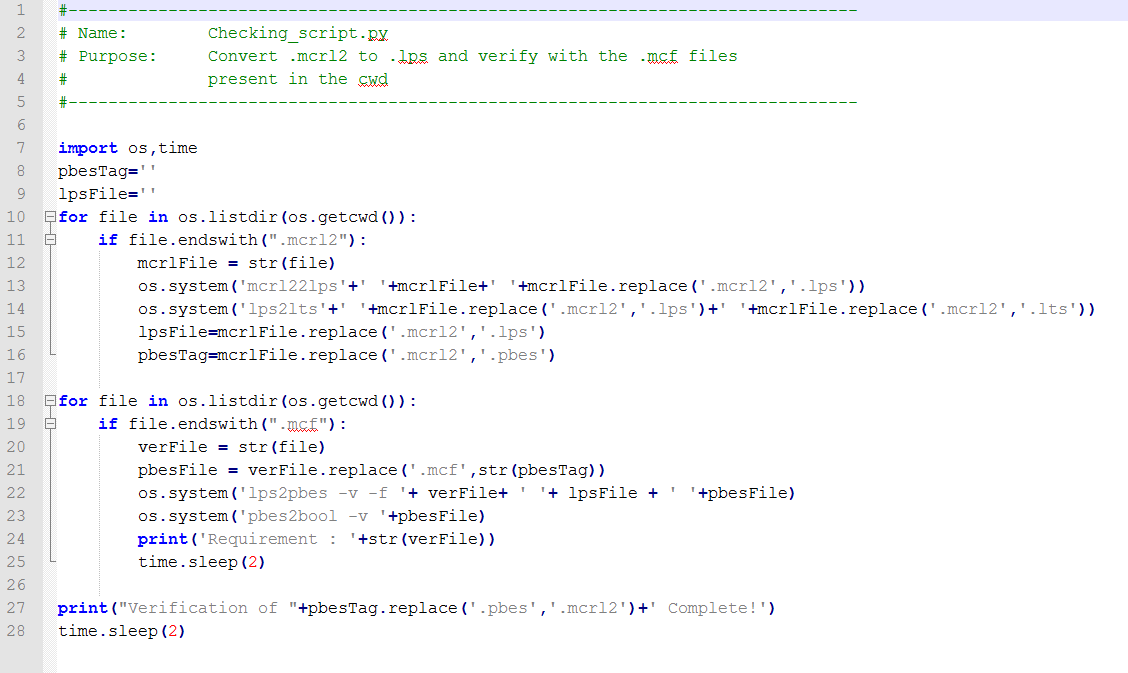
\includegraphics[scale=0.4]{Check_script.PNG}
      \caption{Checking script}
%      \label{figurelabel}
   \end{figure}


\section{Conclusions}

All the formulated requirements listed in Section 8 were evaluated as \emph{true} in the verification process using the mcrl2 toolset for a maximum of four trains. It is concluded that the Automatic Railroad Crossing System satisfies all mentioned requirements.


\section{References}
\begin{enumerate}
\item J. F. Groote and M. R. Mousavi Modeling and Analysis of Communicating Systems 2013. \\
\item mCRL2 201210.1 documentation 
\url{http://www.mcrl2.org/release/user_manual/user.html}
\end{enumerate}

\newpage
\section{System Model}
DO NOT PRINT THIS PAGE. ADD THE CODE FROM THE WORD FILE
\end{document}